\chapter{Standard Model and Supersymmetry}
\label{chap:SMSUSY}

This chapter presents an introduction to the Standard Model (SM) of particle physics, the theory that nowadays best described the subatomic world. In Section \ref{sec:smsusy:sm} a general overview of the SM is given. Section \ref{sec:smsusy:bsm} discusses the limitations of the SM, and some of the theoretical extensions proposed to overcome them. Finally Section \ref{sec:smsusy:susy} focuses on Supersymmetry (SUSY), one of the most promising of these extensions. Throughout this Chapter (as well as in the rest of this thesis) we use Natural units; we will thus use energy units to describe masses, as the speed of light ($c$) and the Plank constant ($\hslash$) are set to unity.


\section{The Standard Model of Particle Physics}
\label{sec:smsusy:sm}

The Standard Model (SM) is a renormalizable gauge quantum field theory based on the group $SU(3) \times SU(2) \times U(1)$. It has been developed in the second half of the 20th century \cite{Glashow:1961tr}\cite{Weinberg:1967tq}\cite{Salam:1980jd}, and since then the description that it gives of the elementary particles and of their interactions has been accurately tested by several experiments. Many experimental discoveries have been guided by the SM predictions, including the discovery of the top quark \cite{Abachi:1994td}\cite{PhysRevLett.74.2626} and up to the latest one, the observation of the Higgs boson at the LHC in July 2012 \cite{Aad:2012tfa}\cite{Chatrchyan:2012xdj}. 

\subsection{Particle Content of the Standard Model}

\subsubsection{Fermions}

In the SM, particles are described as fields excitations; in particular, matter constituents are half-integer spin fields (\textit{fermions}). Fermions are further divided into two categories based on the type of interaction they experience:
\begin{itemize}
\item Leptons experience only the electroweak interaction
\item Quarks experience both the electroweak and the strong interaction
\end{itemize}

Both leptons and quarks come in three generations, and conventionally the numbering of these generations follows an order of increasing mass. While it is possible to observe free leptons, quarks exist only in bound states (\textit{hadrons}); this is because of confinement, discussed in Section \ref{sec:strong}. Hadrons built of three quarks have spin $\frac{1}{2}$ and are named \textit{barions}, while \textit{mesons} are formed by two quarks and have integer spin.


The free lagrangian of a fermion is given by:

\begin{equation}
 \mathcal{L}_{free} = \bar{\psi} \left( i \gamma^{\mu} \partial_{\mu} - m \right) \psi \, , \
 \label{eq:sm:dirac}
\end{equation}

\noindent where $\psi$ is the fermion field, $m$ its mass, $\gamma$ are the Dirac matrices and $\partial_{\mu}$ is the four-vector derivative.

\iffalse
\begin{equation}
\psi_L = \frac{(1 - \gamma_5)}{2} \psi, \qquad\qquad
\psi_R = \frac{(1 + \gamma_5)}{2} \psi
 \label{eq:sm:siLR}
\end{equation}

\begin{equation}
P_L = (1 - \gamma_5)/2, \qquad\qquad
P_R = (1 + \gamma_5)/2
 \label{eq:sm:parity}
\end{equation}
\fi

\subsubsection{Bosons}

Particles with integer spin are referred to as \textit{bosons}. In the SM, force carriers are described through spin-1 fields. Beside force carriers, the SM includes another boson, the Higgs boson, that has spin 0. All the other particles of the SM acquire mass though interaction with the Higgs boson field, as described in Section \ref{sec:smsusy:ew}.

\begin{equation}
\mathcal{L}_{free} = \frac{1}{2} \partial^\mu \phi \partial_\mu \phi + \frac{1}{2} m^2 \phi ^2 ,
\end{equation}

 
\noindent while for a complex scalar field is:

\begin{equation}
\mathcal{L}_{free} =  \partial^\mu \phi \partial_\mu \phi^* +  m^2 \phi \phi^* .
\end{equation}


\noindent On the other hand, a vector field $A^\mu$ with spin 1 obeys the Proca lagrangian if it has mass different from zero

\begin{equation}
\mathcal{L}_{free} =  - \frac{1}{4} F^{\mu \nu}F_{\mu \nu}+  \frac{1}{2} m^2 A^\mu A_\mu ,
\label{eq:lproca}
\end{equation}

\noindent and the Maxwell lagrangian if it has null mass

\begin{equation}
\mathcal{L}_{free} =  - \frac{1}{4} F^{\mu \nu}F_{\mu \nu} ,
\label{eq:lmax}
\end{equation}


\noindent where we have defined $F^{\mu \nu} = \partial^\mu A_\nu - \partial^\nu A_\mu$.

\subsection{Interactions}

The SM describes all the interactions among elementary particles, except for gravity, for which nowadays no renormalizable quantum field theory is known. Table \ref{tab:sm_interazioni} presents a summary of the SM interactions and the properties of the corresponding force carriers. More details about the strong and electroweak sectors are given in the following sections.

\begin{table}[h]
\centering
\begin{tabular}{llccc}
\hline
\multirow{2}*{Interaction} & \multirow{2}*{Carrier} & \multirow{2}*{$\frac{Q}{e}$} & \multirow{2}*{Mass [GeV]} & \multirow{2}*{\textbf{$\alpha$}} \\
 & & & &  \\
\hline
\hline
Strong & Gluons (g)  & 0 & 0 & 10 \\
\hline
Electromagnetic & Photon ($\gamma$) & 0 & 0  & $10^{-2}$ \\
\hline
\multirow{2}*{Weak} & $W^{+}$, $W^{-}$    &  +1, -1 &  	$80.385$ $\pm0.015$ GeV   & \multirow{2}*{$10^{-6}$}\\
 & $Z^{0}$  & 0 &  	$91.1876$ $\pm0.0021$ GeV &  \\
\hline
\end{tabular}
\caption[Interaction in the Standard Model]{Interaction in the Standard Model. Here the different force carriers are listed, with their electric charges and masses \cite{pdg:rev}; $\alpha$ is the coupling constant of the different interactions.}
\label{tab:sm_interazioni}
\end{table}


\subsubsection{Gauge Invariance}

The interaction terms in the SM Lagrangian are introduced by promoting an already existing global symmetry of the Lagrangian ($\theta$) to a \textit{local} one ($\theta(x)$) function of the space-time coordinates. 
In general, given a Lagrangian globally invariant under a symmetry group, the fields transform as:
\begin{equation}
\psi \rightarrow e^{ig\theta_k \tau_k} \psi  
\end{equation}

\noindent where $\tau_k$ are the generators of the group and obey commutation relations: 
\begin{equation}
\left[ \tau_i, \tau_j \right] = i f_{ijk} \tau^k \, . \
\end{equation}

\noindent $f_{ijk}$ is the structure constant of the group and is always zero for Abelian groups. Promoting this invariance to a global one ($\theta_k \rightarrow \theta_k(x)$) implies adding to the theory:
\begin{itemize}
\item A number of massless gauge fields $W^\mu_k$ equal to the number of generators of the symmetry group, that transform as 
\begin{equation}
W^\mu_k \rightarrow W^\mu_k - \partial^\mu \theta_k - g \epsilon_{klm} \theta^m W^\mu_m 
\end{equation}
\item A covariant derivatibe: 
\begin{equation}
D^\mu = \partial^\mu + ig\tau^kW^\mu_k 
\end{equation}

\noindent that substitutes the standard derivative in the Lagrangian
\item A free Lagrangian for the vector fields as in Eq. \ref{eq:lproca}, with:
\begin{equation}
F^{\mu \nu}_k = \partial_\mu W_k^\nu - \partial_\nu W_k^\mu - g f_k^{lm} W^\mu_l W^\nu_m
\end{equation}
\noindent The last term, of second order in the field, is present only for non-Albelian symmetry groups. 
\end{itemize}


The SM is a theory invariant under $SU(3)_\mathrm{C} \times SU(2)_\mathrm{L} \times U(1)_\mathrm{Y}$. Imposing local invariance under $SU(3)_\mathrm{C}$ leads to the theory of strong interactions, while $SU(2)_\mathrm{L} \times U(1)_\mathrm{Y}$ is the symmetry whose breaking gives origin to the electroweak interactions. 

\subsubsection{Strong Interaction}
\label{sec:strong}

Quantum Chromo-Dynamics (QCD) is the theory that describes strong interactions, and it is invariant under the symmetry group $SU(3)_\mathrm{C}$, where the subscript C refers to the color, the quantum number associated with these interactions; this can assume three possible values denoted with red, blue and green. The observable stated (hadrons) are color singlets, while quarks (anti-quarks) carry only one color (anti-colr) charge. Since the symmetry group is non-Abelian, also the corresponding eight gauge bosons (\textit{gluons}) carry a color charge (bi-color, with one color and one different anti-color) and therefore interact not only with quarks but also among themselves. Since $SU(3)_\mathrm{C}$ is believed to be an exact symmetry,  gluons are massless. 

The renormalization of a gauge theory leads to the definition of \textit{running coupling constants}, whose value depends on the energy scale where they are evaluated. In QCD, at leading order the dependence of the coupling constant from the energy scale is given by:

\begin{equation}
\alpha_\mathrm{s}(Q^2)=\frac{1}{b\log{\frac{Q^2}{\Lambda_\mathrm{QCD}^2}}} \quad \quad b = \frac{11N_\mathrm{C}-2n_\mathrm{f}}{12\pi}
\label{eq:alfaQCD}
\end{equation}

\noindent where $N_\mathrm{C}$ is the number of colors, $n_\mathrm{f}$ is the number of quark flavors that are active (i.e. whose mass is lower than the energy scale) and $\Lambda_\mathrm{QCD}$ is the infrared cutoff scale that sets the limit of validity of the perturbative approximation. In QCD $N_\mathrm{C} = 3$, so for $n_\mathrm{f}<16$ the coupling constants decreases with the increase of the energy scale of the process considered. This structure has important consequences on the properties of quarks and gluons:

\begin{itemize}
\item At high $Q^2$ ($\rightarrow$ small distances), $\alpha_\mathrm{s}$ becomes small enough for the perturbative approximation to be correct. In this case quarks and gluons behave as free particles (\textit{asymptotic freedom}) \cite{PhysRevLett.30.1343}\cite{PhysRevLett.30.1346}.
\item When the momentum transfer is small ($\rightarrow$ large distances) $\alpha_\mathrm{s}$ is large; this gives rise to \textit{confinement}: quarks can not be observed as isolated particles, as it is not possible to extract individual quarks from hadrons. When the distance between two quarks is increased, the potential energy increases as well, up to the point when is energetically more favorable to create from the vacuum a quark-antiquark pair and thus a new hadron is formed.
\item In a collider experiment, quarks and gluons will create a collimated spray of hadrons (\textit{jets})
\end{itemize}



\subsubsection{Electroweak Interaction and Higgs Physics}
\label{sec:smsusy:ew}

\begin{figure}
\centering
\subfigure[]{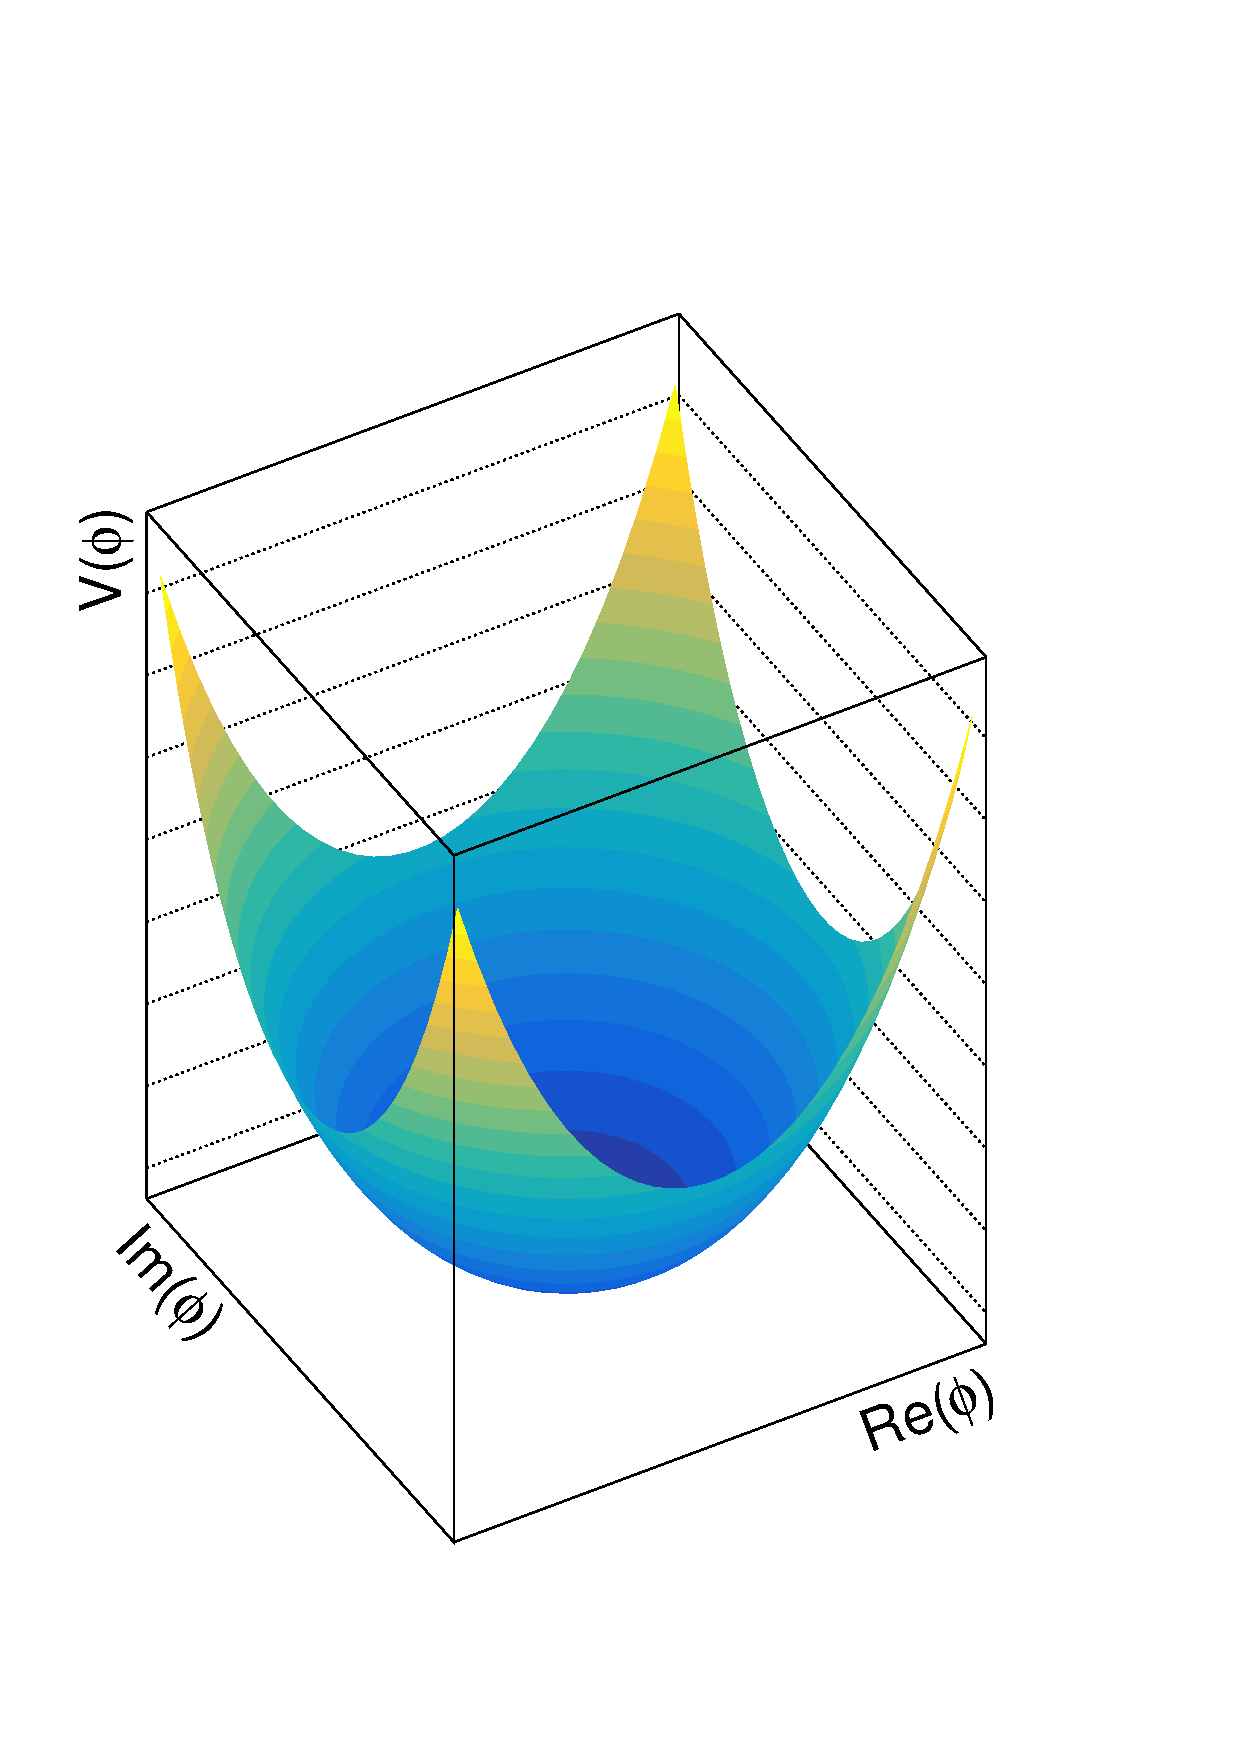
\includegraphics[width=0.49\textwidth]{produce_plots/sm/higgs_posmu2.pdf}}
\subfigure[]{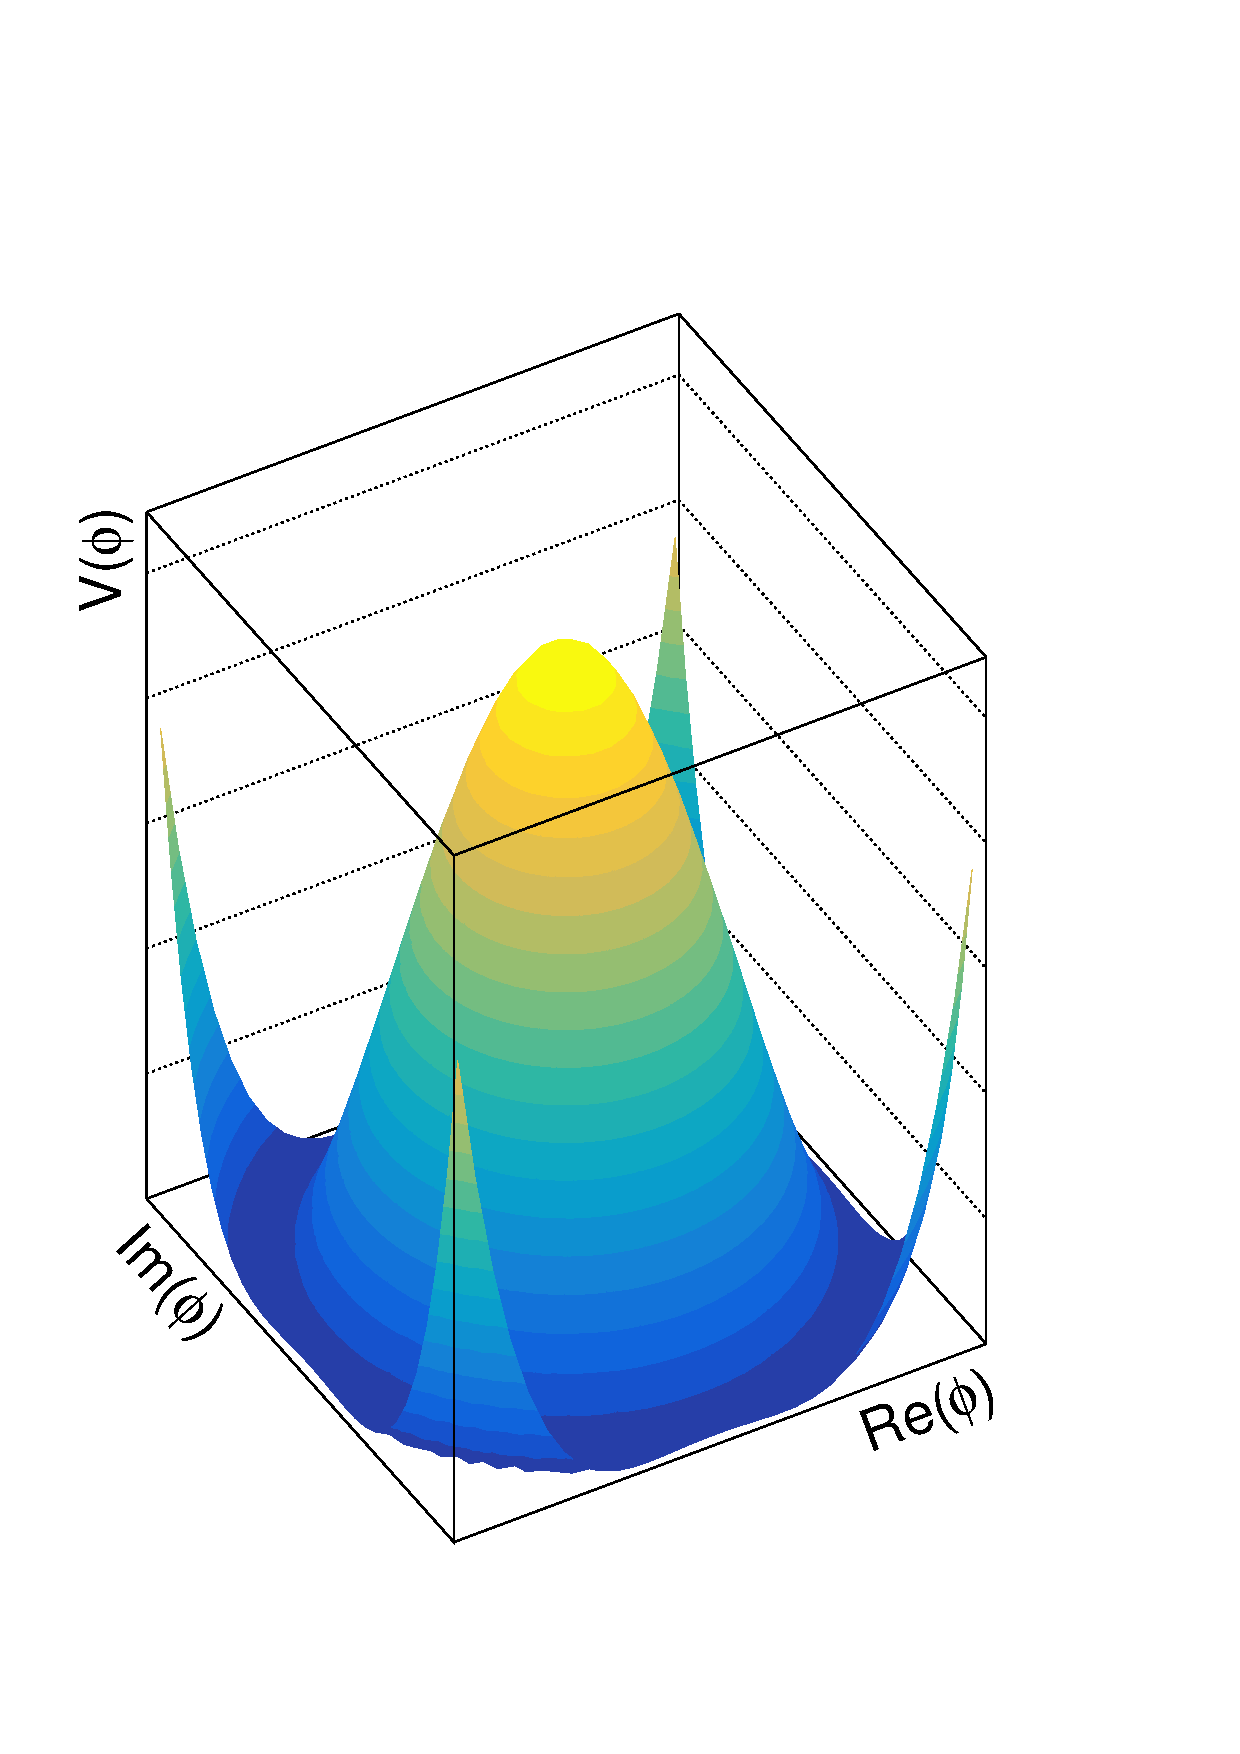
\includegraphics[width=0.49\textwidth]{produce_plots/sm/higgs_negmu2.pdf}}
\end{figure}

\section{Limits of the Standard Models and its Extensions}
\label{sec:smsusy:bsm}




\section{Supersymmetry}
\label{sec:smsusy:susy}

